\documentclass[10pt, conference]{IEEEtran}
\IEEEoverridecommandlockouts
% The preceding line is only needed to identify funding in the first footnote. If that is unneeded, please comment it out.
\usepackage{cite}
\usepackage{amsmath,amssymb,amsfonts}
\usepackage{algorithmic}
\usepackage{graphicx}
\usepackage{textcomp}
\usepackage{xcolor}
\def\BibTeX{{\rm B\kern-.05em{\sc i\kern-.025em b}\kern-.08em
    T\kern-.1667em\lower.7ex\hbox{E}\kern-.125emX}}

\begin{document}

\title{Assignment 1\\
% {\footnotesize \textsuperscript{*}Note: Sub-titles are not captured in Xplore and
% should not be used}
% \thanks{Identify applicable funding agency here. If none, delete this.}
}

\author{\IEEEauthorblockN{Andre van der Merwe}
% \IEEEauthorblockA{\textit{dept. name of organization (of Aff.)} \\
% \textit{name of organization (of Aff.)}\\
% City, Country \\
% email address or ORCID}
}

\maketitle

% \begin{abstract}
%     This document is a model and instructions for \LaTeX.
%     This and the IEEEtran.cls file define the components of your paper [title, text, heads, etc.]. *CRITICAL: Do Not Use Symbols, Special Characters, Footnotes, 
%     or Math in Paper Title or Abstract.
% \end{abstract}

% \begin{IEEEkeywords}
%     component, formatting, style, styling, insert
% \end{IEEEkeywords}

% \section{Introduction}
% This document is a model and instructions for \LaTeX.
% Please observe the conference page limits. 

\begin{table}[h!]
    % \caption{\textbf{Continuous Features}}
    \caption{Continuous Features}
    \begin{center}
    \begin{tabular}{|c||c|c|c|c|c|c|c|c|c|c|}
        \hline
        \textbf{Features}&\textbf{Count}&\textbf{\% Miss.}&\textbf{Card.}&\textbf{Min.}&\textbf{$1^{st}$ Qrt.}&\textbf{Mean}&\textbf{Median}&\textbf{$3^{rd}$ Qrt.}&\textbf{Max}.&\textbf{Std Dev.}\\
        \hline
        %   	                    Count   % Miss     Card.    Min         1st Q       Mean          Median      3rd Q       Max         Std Dev
        \textbf{Area}               &13611  &0.0       &12011   &20420      &36328      &53048.284549 &44652      &61332      &254616     &29324.095717\\
        \textbf{Perimeter}          &13611  &0.0       &13351   &524.736    &703.5235   &855.283459   &794.941    &977.213    &1985.37    &214.289696\\
        \textbf{MajorAxisLength}    &13611  &0.0       &13543   &183.601165 &253.303633 &320.141867   &296.883367 &376.495012 &738.860153 &85.694186\\
        \textbf{MinorAxisLength}    &13611  &0.0       &13543   &122.512653 &175.848170	&202.270714   &192.431733 &217.031741 &460.198497 &44.970091\\
        \textbf{AspectRation}       &13611  &0.0       &13543   &1.024868   &1.432307   &1.583242     &1.551124   &1.707109	  &2.430306   &0.246678\\
        \textbf{Eccentricity}       &13611  &0.0       &13543   &0.218951   &0.715928   &0.750895     &0.764441	  &0.810466	  &0.911423   &0.092002\\
        \textbf{ConvexArea}         &13611  &0.0       &12066   &-30        &36714.5    &53765.692602 &45178      &62294      &263261     &29778.009358\\
        \textbf{EquivDiameter}      &13611  &0.0       &12012   &0.161417   &215.068003 &476.254106   &238.438026 &279.452162 &3014441    &25836.865632\\
        \textbf{Extent}             &13611  &0.044082  &13529   &0.555315   &0.718641   &0.749747     &0.759874   &0.786852	  &0.866195	  &0.049085\\
        \textbf{Solidity}           &13611  &0.0       &13526   &0.919246	&0.985670	&0.987143     &0.988283   &0.990013   &0.994677   &0.004660	\\
        \textbf{Roundness}          &13611  &0.0       &13543   &0.489618   &0.832096   &0.873282     &0.883157   &0.916869   &0.990685   &0.059520\\
        \textbf{Compactness}        &13611  &0.132246  &13525   &0.640577	&0.762577	&0.799886	  &0.801291	  &0.834270   &0.987303   &0.061684\\
        \textbf{ShapeFactor1}       &13611  &0.0       &13543   &0.002778   &0.005900   &0.006564	  &0.006645   &0.007271   &0.010451   &0.001128\\
        \textbf{ShapeFactor2}       &13611  &0.0       &13543   &0.000564	&0.001154	&0.001716	  &0.001694	  &0.002170   &0.003665   &0.000596\\
        \textbf{ShapeFactor3}       &13611  &0.0       &13543   &0.410339   &0.581359	&0.643590     &0.642044	  &0.696006	  &0.974767   &0.098996\\
        \textbf{ShapeFactor4}       &13611  &0.0       &13611   &0.695579	&1.614151	&2.368097	  &2.368757   &3.115695	  &3.966119   &0.871619\\
        \textbf{ShapeFactor5}       &13611  &0.0       &13543   &0.947687   &0.993703   &0.995063	  &0.996386	  &0.997883   &0.999733   &0.004366\\
        \textbf{ShapeFactor6}       &13611  &0.036735  &13606   &0.000466	&45.258826	&89.358603	  &88.76667   &134.273148 &178.985023 &51.838555\\
        \textbf{Sort order}         &13611  &0.0       &13611   &0.000089   &0.248187   &0.500271     &0.50381    &0.750096   &0.999985   &0.287926\\

        \hline
    \end{tabular}
    \label{continuous features}
    \end{center}
\end{table}

\begin{table}[h!]
    % \caption{\textbf{Continuous Features}}
    \caption{Categorical Features}
    \begin{center}
    \begin{tabular}{|c||c|c|c|c|c|c|c|c|c|}
        \hline
        \textbf{Features}&\textbf{Count}&\textbf{\% Miss.}&\textbf{Card.}&\textbf{Mode}&\textbf{Mode Freq.}&\textbf{Mode \%}&\textbf{$2^{nd}$ Mode}&\textbf{$2^{nd}$ Mode Freq.}&\textbf{$2^{nd}$ Mode \%}\\
        \hline
        %   	                    Count   % Miss     Card.    Mode      Mode Freq   Mode %        2nd Mode    2nd Mode Freq  2nd Mode %
        \textbf{Constantness}       &13611  &0.0       &2       &1        &12289      &90.287268     &0          &1322         &9.712732\\
        \textbf{Colour}             &13611  &0.044082  &5       &brown    &6115       &44.926897    &black      &3541          &26.015723\\
        \textbf{Class}              &13611  &0.124899  &8       &DERMASON &3542       &26.02307     &SIRA       &2634          &19.351995\\

        \hline
    \end{tabular}
    \label{categorical features}
    \end{center}
\end{table}

\begin{table}[h!]
    \caption{Hyperparameter tuning for Classification tree}
    \begin{center}
        \begin{tabular}{|c||c|c|c|c|}
            % \hline
            % \textbf{Max depth}
            % \cline{0-5}
                        & \textbf{2} & \textbf{3} & \textbf{4} & \textbf{5} \\
            \hline
            \textbf{8}  & 93.08315 & 93.08315 & 93.06107 & 93.05372 \\
            \textbf{9}  & 93.48786 & 93.48786 & 93.47314 & 93.46578\\
            \textbf{10} & 93.46578 & 93.45107 & 93.41428 & 93.39220\\
            \textbf{11} & 93.42899 & 93.43635 & 93.39956 & 93.41428\\
            \textbf{12} & 93.39220 & 93.39956 & 93.37013 & 93.36277\\
        \end{tabular}
    \end{center}
\end{table}

% \begin{figure}[b!]
%     \centerline{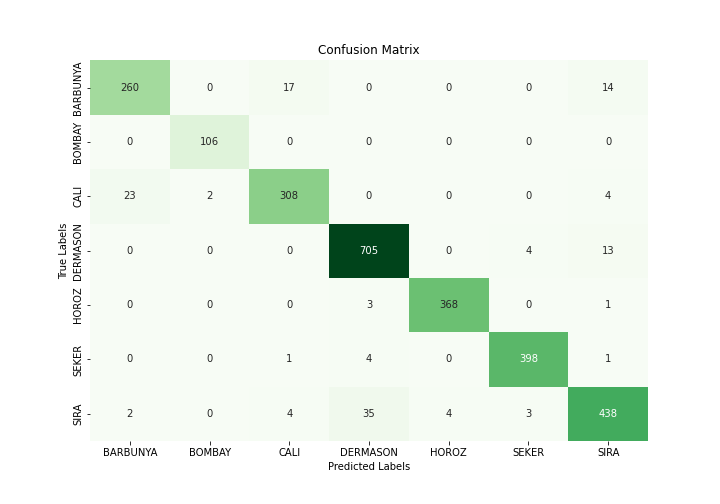
\includegraphics[scale=0.3]{../Plots/Classification tree confusion matrix.png}}
%     \caption{Classification tree confusion matrix}
%     \label{clf confusion matrix}
% \end{figure}

\end{document}